\section{Nonmonotonic Rule Learning}\label{sec:nmrulelearn}
So far we have considered approaches that learn Horn rules. However,  Horn rules are not sufficiently expressive for representing incomplete human knowledge, and they are inadequate for capturing
exceptions. Thus, the rules extracted from the existing KGs can potentially %they %herefore, they 
predict erroneous facts as illustrated in Section~\ref{sec:intro}. 

In this section, we provide an overview of approaches for nonmonotonic rule learning extraction from incomplete data. 

\subsection{Revision-based Method}
In \cite{DBLP:conf/semweb/Gad-ElrabSUW16,ilp2016} a revision-based approac for extracting exception-enriched (i.e., nonmonotonic)  rules from KGs has been proposed, which accounts for the KG incompleteness and their large size. 
% In \cite{ilp2016} the results from \cite{DBLP:conf/semweb/Gad-ElrabSUW16} to KGs in their original relational form.
More specifically, in these works the KG completion problem from Definition~\ref{def:kgcomp} is treated 
as a \emph{theory revision} task, where, given a KG and a set of (previously learned) Horn rules, the goal is to revise this set to obtain a set of nonmonotonic rules, such that the revised ruleset is more accurate for link prediction than the original one. Essentially, one is interested in tackling a theory revision problem, in which, as possible revision operations, one is allowed to add only negated atoms to the antecedents of the rules. 

This approach combines standard relational association rule mining techniques with a FOIL-like supervised learning algorithm \cite{foil}, which is used to detect exceptions. More specifically, the proposed method proceeds in four steps as follows (see Figure~\ref{fig:iswc_process}).

% \cite{gad2016} and its successor RUMIS~\cite{rumis} have been developed specifically to learn nonmonotonic rules from the large KGs, taking into account the OWA and the huge size of the KG. 
% Both %\cite{gad2016} and RUMIS try to 
% %learn exceptions from a learned rules set % in the KG 
% %by revising % the set of Horn rules $R_H$ extracted from the KG
% % into a nonmonotonic set $R_{MN}$ by
% learn exceptions starting with a learned Horn rules set and revise it by  
% adding at most one negated atom to each rule at a time. The revision is constructed such that the average quality of the Horn rule set is maximized, while the conflict among the predictions of the rules are minimized. To estimate this conflict ratio, the negative predictions are materialized. To this end, % herefore,
% % they introduce 
% the notion of an auxiliary rule for a given rule $r:H \leftarrow B, \naf E$ has been introduced as follows: % , concretely, for a rule 
% %, the auxiliary version is 
% $r^{aux}:\mi{not\_H} \leftarrow B, E$ where $\mi{not\_H}$ is a fresh predicate indicating that $H$ will not be derived by this rule. The number of grounded pairs $\tuple{H,\mi{not\_H}}$ in the answer set generated by the rule set, the auxiliary rules and the KG indicates the degree of conflict.

\begin{figure}[t]
\centering
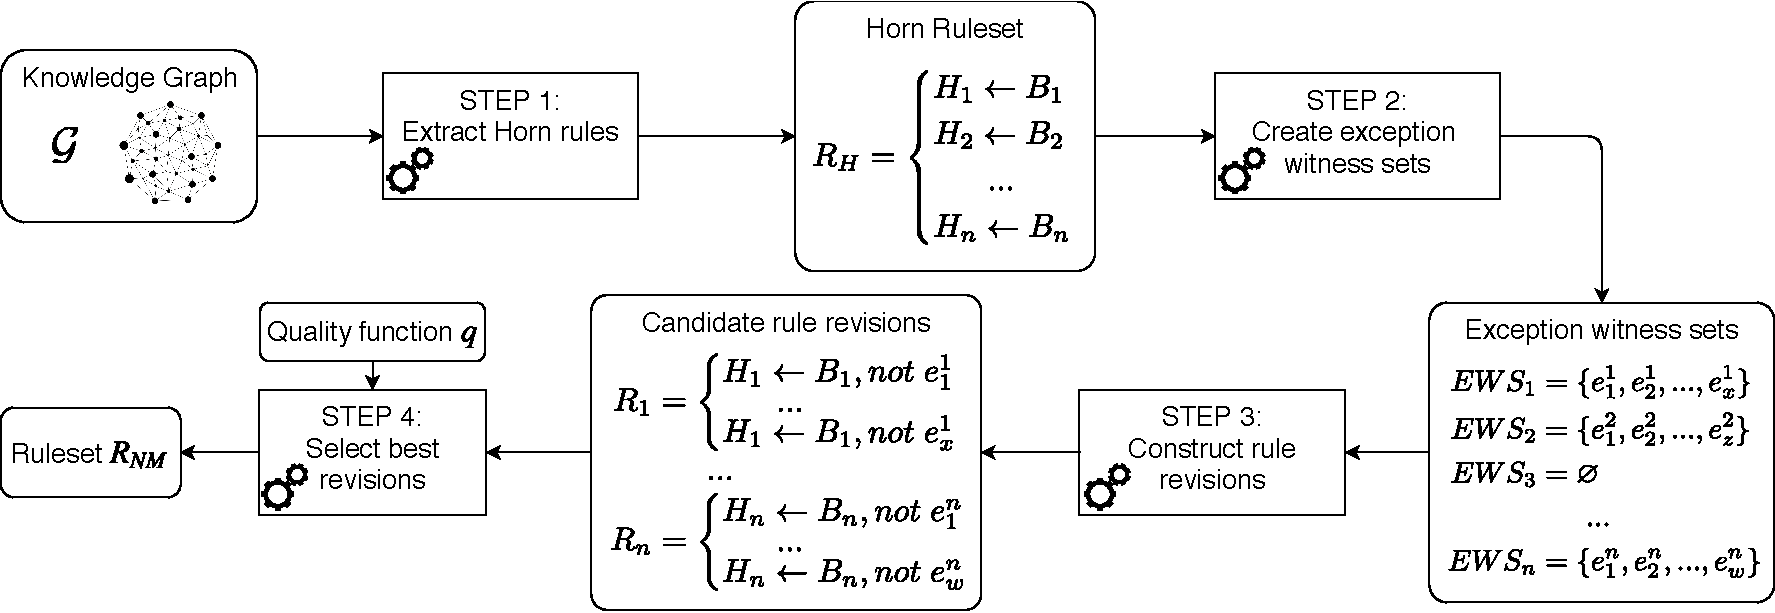
\includegraphics[width=1\textwidth]{figures/overview_new}
\caption{Rule revision process by~\cite{gad2016,rumis}.}
\label{fig:iswc_process}
\end{figure}

%Figure shows an overview of the rule revision steps. % 
The first step concerns the extraction of Horn rules from the KG relying on any existing Horn rule extraction method, such as \cite{amie}.
 In the second step, for every Horn rule the \textit{normal} and \textit{abnormal} substitutions are determined, i.e., substitutions that satisfy (resp. do not satisfy) the considered rule. Thi, the so-called \emph{exception witness sets} are computed, i.e., sets of predicates that are potentially involved in explaining why abnormal substitutions fail to follow the rule. Formally, the normal and abnormal sets are respectively defined as follows:
\begin{itemize}
\item $NS(r, \cG) = \{\theta \mid head(r)\theta, body(r)\theta \subseteq \cG\}$
\item $ABS(r, \cG) = \{\theta \mid body(r)\theta \subseteq \cG , head(r)\theta \notin \cG\}$\\
where $\theta: \mathcal{V} \rightarrow \cC$.
\end{itemize}
where $\mathcal{V}$ is the set of variables appearing in $r$. 

Third, candidate rule revisions are constructed by adding to a rule body a single exception at a time. The quality measures for nonmonotonic rules are devised to quantify their strength w.r.t the KG. Importanly, the crosstalk between the rules through is considered via the novel \emph{partial materialization} technique instead of revising rules in isolation. Fourth, the rule revisions are ranked according to these measures to determine a ruleset that not only describes the data well but also shows a good predictive power by taking exceptions into account. 



\begin{example}
Consider the KG $\cG$ and $r_1$ from Figure~\ref{rdf} as before, the normal set for $r_1$ is $NS(r_1,\cG)=\{\theta_1, \theta_2 ,\theta_3\}$, where $\theta_1 = \{X/brad, Y/ann, Z/berlin\}$,\\  $\theta_2 = \{X/john, Y/kate, Z/chicago\}$ and $\theta_3 = \{X/sue, Y/li, Z/beijing\}$.\\ and the abnormal set, $ABS(r_1,\cG)=\{\theta_4,\theta_5, \theta_6\}$, \\such that $\theta_4=\{X/bob, Y/alice, Z/berlin\}$,  $\theta_5=\{X/clara, Y/dave, Z/chicago\}$, and $\theta_6=\{X/mat, Y/lucy, Z/amsterdam\}$.
\qed
\end{example}



In the third step the exception witness sets (EWSs) are constructed. The Exception Witness Set (EWS) of $r$ with respect to the KG and a variavle $X\in V$ is the maximal set of predicates $EWS(r,\cG,\mathcal{X}) = \{p_1,...,p_k\}$ such that:
\begin{itemize}
\item $\forall i \in \{1,..,k\} : \exists \theta \in ABS(r, \cG)\ s.t.\ p_i(\mathcal{X}\theta) \in \cG$, and 
\item $\forall \theta \in NS(r,\cG) :  p_1(\mathcal{X}\theta), ...,p_k(\mathcal{X}\theta) \notin \cG$
\end{itemize}

\begin{example}
Recalling $\cG$ and $r_1$, the exceptions witness sets for both variable $X$ and $Y$ are $EWS(r_1,\cG,\{X\}) = \{artist\}$ and $EWS(r_1,\cG,\{Y\}) = \{researcher\}$, respectively.
\qed
\end{example}
For each rule $r \in \cR_H$, the EWSs are collected in one set $EWS(r,\cG)$ containing all of its exception candidates. 
%\[EWS(r,\cG)=\bigcup_{\forall\mathcal{X}\subseteq \mathcal{V}}EWS(r,\cG,\mathcal{X})\] 

After the exception witness sets are computed for every rule, the search for the best possible revision is performed relying on the following exception scoring functions:
\begin{itemize}
\item \textbf{Naive}: It is the direct way of choosing the revision using only some standard measure such as confidence or conviction.
\item \textbf{PM}: Intuitively, the idea behind the \textit{partial materialization} is to rank candidate revisions based on its extension with predictions produced by other rules in $R_H$ (\ie partially materialized); hence, ensuring a cross-talk between the rules.
\item \textbf{OPM}: The \textit{ordered partial materialization} is similar to \textbf{PM}, but only materialize the rules of $\cR_{H}$ with higher quality than the current rule.
\item \textbf{OWPM}: The \textit{ordered weighted partial materialization} distinguishes between the original facts in the KG and the partial materialization facts by assigning a weight for the materialized facts inherited from the rules used to generate them. Materializing facts with weights from the rules and exiting KG is the concern of probabilistic deductive reasoning tools such as Problog~\cite{problog2007,problog2015}. %or DLV~\cite{dlv2006}.\gad{no sure about DLV citation}
\end{itemize}



\subsection{Method Guided by Embedding Models}
  \begin{figure}[t]
\centering
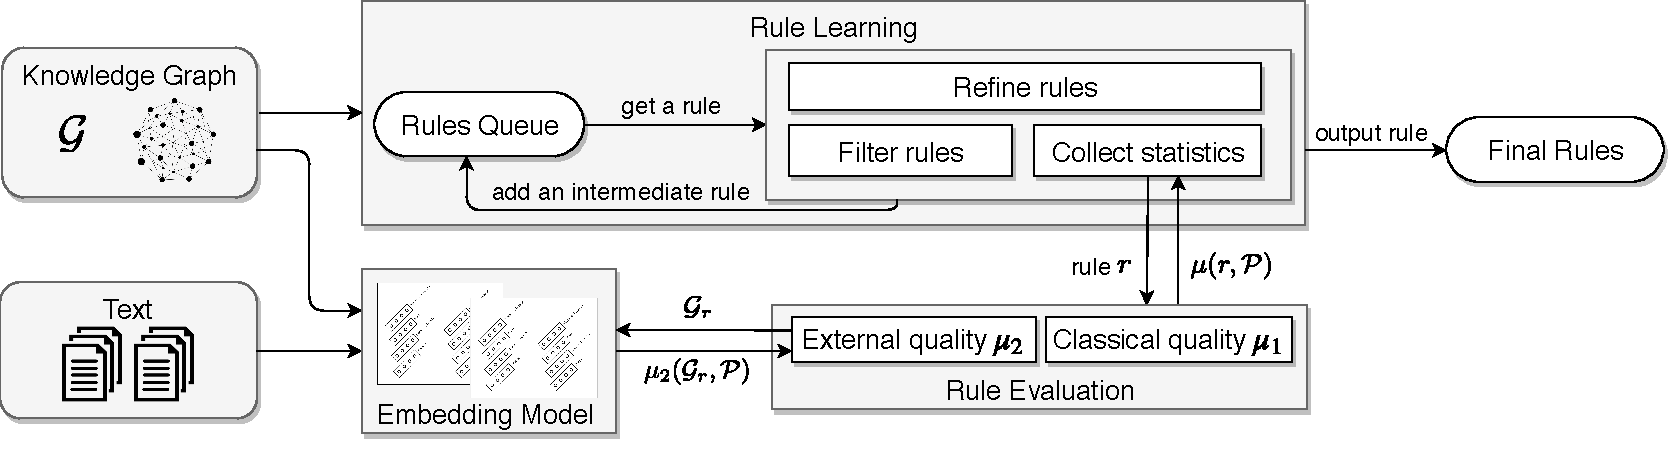
\includegraphics[width=1\textwidth]{figures/rules_overview_H.pdf}
\caption{RulES system.}
\label{fig:system}
\end{figure}


An alternative relational learning method for KG completion is to learn representations (i.e. embeddings) of entities and relations from a given KG possibly enriched with additional information sources (e.g., text) with the purpose of estimating the likelihood of unseen facts (see \cite{Wang2017} for overview). However, the predictions produced by such approaches are not interpretable~\cite{Shakerin2018}. 

RulES~\cite{thinh2018} established a framework to benefit from the advantages of these models while constructing nonmontonic rule sets. In particular, RulES iteratively construct rules over a KG and collect statistics from a precomputed embedding model allowing assessing the quality of (partially constructed) rule candidates. 

To explain the core of RulES, let $\cG$ be a KG over the signature $\Sigma_{\cG}=(\cR_\cG,\cC_\cG)$. 
A \emph{probabilistic KG} $\cP$ is a pair $\cP = (\cG,f)$ 
where $f:\cR_\cG\times \cC_\cG \times \cC_\cG\rightarrow [0,1]$ is a probability function over the facts over $\Sigma_{\cG}$ such that for each atom $a \in \cG $ it holds that $f(a) \geq \theta $, where $\theta$ is a correctness threshold.

The goal of RulES is to learn rules that not only describe the available graph $\cG$ well, but also predict highly probable facts based on the function $f$ which in that case relies on embeddings of the KG. For that, it utilizes a hybrid rule quality function:
\begin{align*}
	\mu(r,\cP)= (1 - \lambda)\times \mu_1(r,\cG) + \lambda \times \mu_2(\cG_r,\cP).
\end{align*}

where $\lambda$ is a weight coefficient and $\mu_1$ is any classical quality measure of $r$ over $\cG$ such that $\mu_1: (r,\cG) \mapsto \alpha \in  [0,1]$ (\eg \textit{standard confidence} or \textit{PCA confidence}~\cite{amie}). 
$\mu_2$ measures the quality of $\cG_r$ (\ie the extension of $\cG$ resulting from executing rule $r$) based on $\cP$ such that
 $\mu_2{:}\, (\cG_r,\cP) \mapsto  \alpha \,{\in}\, [0,1]$. To this end, $\mu_2$ is defined as the average probability of the newly predicted facts in $\cG_r$, formally defined as:
\begin{align*}
	\mu_2(\cG_r,\cP) = (\Sigma_{a\in \cG_r\backslash \cG} f(a)) /
				|\cG_r \backslash \cG|.
\end{align*}
  \gad{Not sure if we should add more here regarding $\mu_2$}



RulES takes as input a KG, possibly a text corpus, and a set of user specified parameters that are used to terminate rule construction.
These parameters include an embedding weight $\lambda$, 
a minimum threshold 
for $\mu_1$,  
a minimum rule support $\textit{r-supp}$ 
and other \emph{rule-related} parameters such as a maximum number of positive %$\mi{max\_pos}$ 
and negative 
atoms allowed in $\mi{body(r)}$.
The KG and text corpus are used to train the embedding model that in turn is used to construct the probabilistic function $f$.{}
The rules $r$ are constructed in the iterative fashion, starting from the head, by adding atoms to its body one after another until at least one of the termination criteria (that depend on $f$) is met.
In parallel with the construction of $r$ the quality $\mu(r)$ is computed.

Figure~\ref{fig:system} demonstrates a high level architecture of RulES, where arrows depict information flow between blocks.
The \emph{Rule Learning} block constructs rules over the input KG similar to rule construction described in Section~\ref{subsec:rule_const}, \emph{Rule Evaluation} supplies it with quality scores $\mu$ for rules $r$, using $\cG$ and $f$, where $f$ is computed by the \emph{Embedding Model} block from $\cG$ and text. Finally, the system produces a set of nonmontonic rules suitable for KG completion.



 

